\section{Overall use cases}

\begin{figure}[H]
  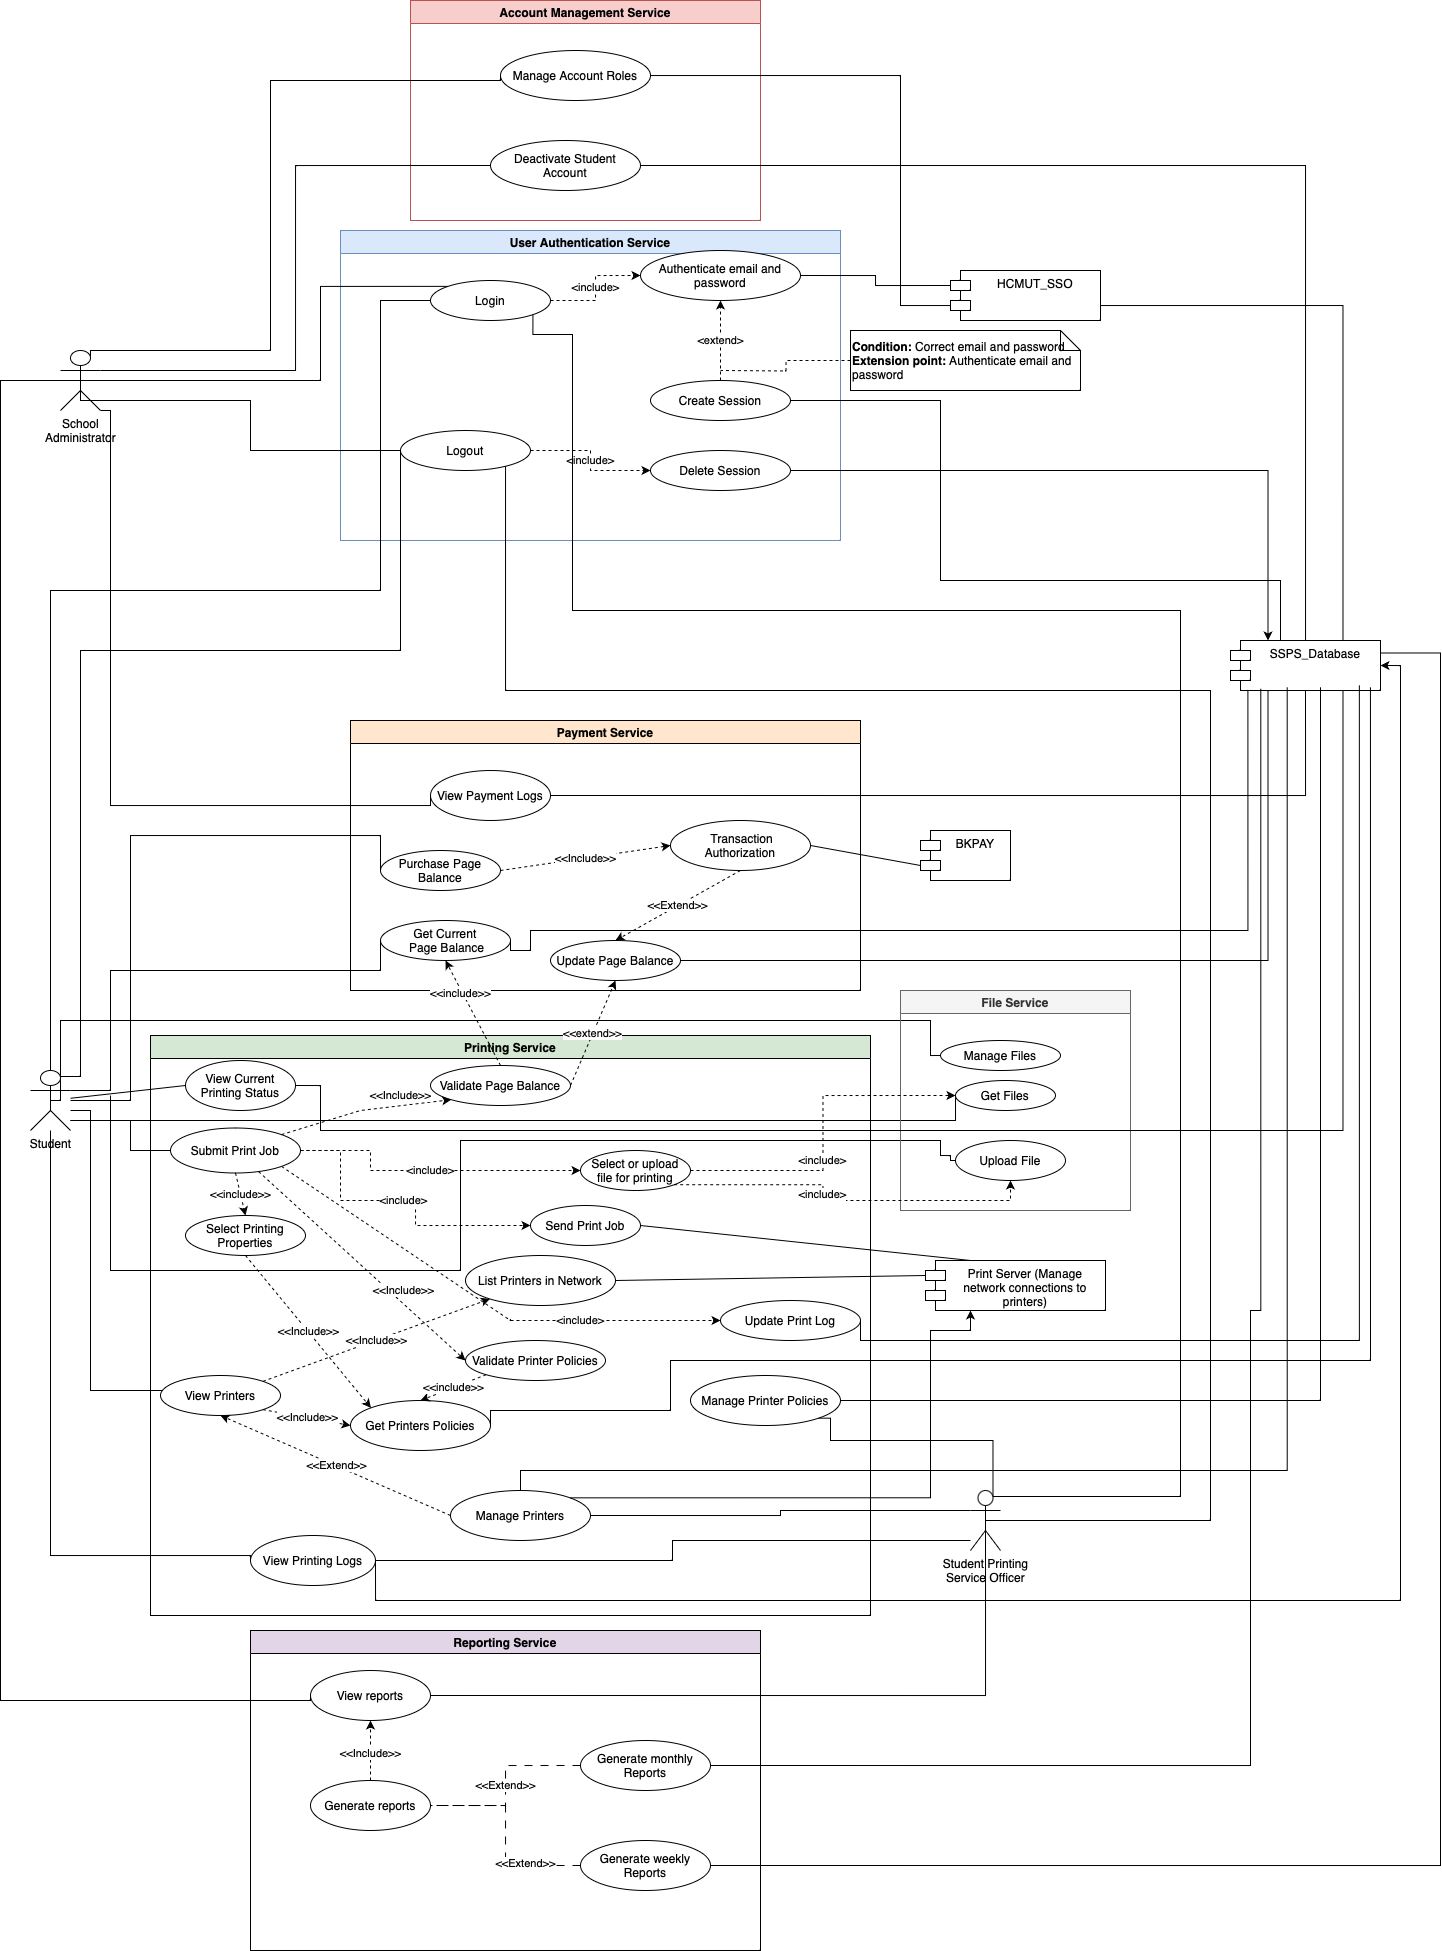
\includegraphics[max width=0.9\linewidth]{chapters/3. use-case-diagram/overall-use-case-diagram.png}
  \caption{Use case of the whole system}%
\end{figure}

\

For the full diagram, check out the following links: \href{https://drive.google.com/file/d/1WRi-N7SIQ2TsGwEkwdd48GqCGhodFedc/view?usp=drive_link}{Draw.io diagram}, \href{https://drive.google.com/file/d/1CZHHrL5VMrCAE1oMELBysDtHTPctMH6j/view?usp=drive_link}{Full resolution image}.

\

The whole system of SmartStudentPrintingService contains 5 modules:

\begin{itemize}
\item \textbf{Account Management Service:} This module is responsible for managing user accounts within the system, specifically catering to the administrative functions. It allows administrators to create, redefine, deactivate, or delete user accounts, including those of students and Student Printing Service Officers (SPSOs).

\item \textbf{User Authentication Service:} The User Authentication Service ensures secure access to the system by verifying the identity of users. It utilizes the HCMUT\_SSO authentication service to authenticate students and other users before granting access to the system's features.

\item \textbf{Payment Service:} This module facilitates online payments for students to purchase additional printing pages. It integrates with payment systems like BKPay, allowing students to extend their page balance for printing. The service ensures that purchased page balances are reflected immediately within the application.

\item \textbf{Printing Service:} The Printing Service is a core component that enables students to initiate and manage print jobs. It handles the upload and printing of documents, printer selection, specifying printing properties (e.g., paper size, page range), and maintaining a history of printing actions. It also enforces page balance checks and notifications when balance is depleted.

\item \textbf{File Service:} The File Service is responsible for securely handling and storing uploaded document files by students. It ensures that files are accessible only to the respective student who uploaded them and authorized personnel, such as SPSOs. This module plays a crucial role in maintaining data privacy and security.

\item \textbf{Reporting Service:} The Reporting Service automatically generates and stores reports summarizing system usage. It compiles statistics on page usage, the number of students using the service, and provides comparisons with previous time intervals (monthly and yearly). These reports are valuable for assessing resource utilization and making informed decisions about the printing service.
\end{itemize}

\section{Detailed use cases}

\subsection{User Authentication and Session Management Use Cases}

\subsubsection{Use-case diagram}

\begin{figure}[H]
  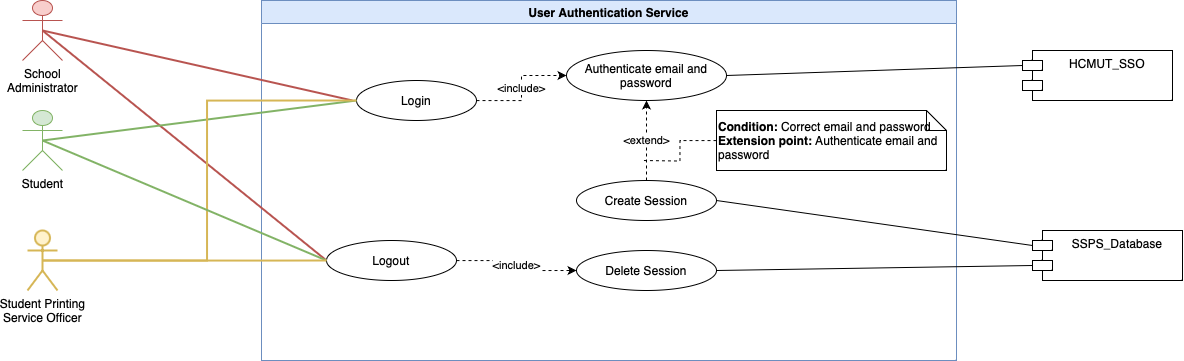
\includegraphics[max width=0.9\linewidth]{chapters/3. use-case-diagram/authentication-use-case-diagram.png}
  \caption{Use case of the whole system}%
\end{figure}

\subsubsection{Table format: Login Feature}

\begin{table}[H]
\begin{tabular}{|p{5cm}|p{9cm}|}
\hline
\textbf{Use Case Name} & User Login and Session Management \\
\hline
\textbf{Actors} & Student User, HCMUT\_SSO, User Authentication Service, SSPS\_Database \\
\hline
\textbf{Description} & Allows a registered user to log in and maintain a user session. \\
\hline
\textbf{Trigger} & User clicks on the Login button on the navbar. \\
\hline
\textbf{Preconditions} & The system is running and accessible. The user has valid HCMUT\_SSO credentials. \\
\hline
\textbf{Postconditions} & User is logged in, and a user session is created in SSPS\_Database. \\
\hline
\textbf{Normal Flows} & 
1. User get redirected to HCMUT\_SSO for authentication. \\
&2. User enters HCMUT\_SSO username and password on the HCMUT\_SSO login page. \\
&3. HCMUT\_SSO authenticates user credentials and redirects back to SSPS upon successful login. \\
&4. SSPS creates a user session. \\
&5. User gains access to system features. \\
\hline
\textbf{Exceptions} & 
From 2a. If the user's HCMUT\_SSO credentials are invalid, display an error message. \\
&From 3a. If the user cancels the login on the HCMUT\_SSO page, display an error message and do not create a user session. \\
\hline
\end{tabular}
\caption{User Login and Session Management Use Case}
\end{table}

\subsubsection{Table Format: Logout Feature}

\begin{table}[H]
\begin{tabular}{|p{5cm}|p{9cm}|}
\hline
\textbf{Use Case Name} & User Logout and Session Termination \\
\hline
\textbf{Actors} & Student User, User Authentication Service, SSPS\_Database \\
\hline
\textbf{Description} & Allows a registered user to log out and terminate their user session. \\
\hline
\textbf{Trigger} & User clicks on the user avatar on navbar and click on the "Logout" button. \\
\hline
\textbf{Preconditions} & User is logged in with an active user session. \\
\hline
\textbf{Postconditions} & User is logged out, and the user session is removed from SSPS\_Database. \\
\hline
\textbf{Normal Flows} & 
1. System terminates the user's session. \\
&2. User is logged out and no longer has access to system features. \\
\hline
\textbf{Exceptions} & None \\
\hline
\end{tabular}
\caption{User Logout and Session Termination Use Case}
\end{table}

\subsection{Submit Printing Job and Printer Management}

\subsubsection{Use-case diagram}

\begin{figure}[H]
  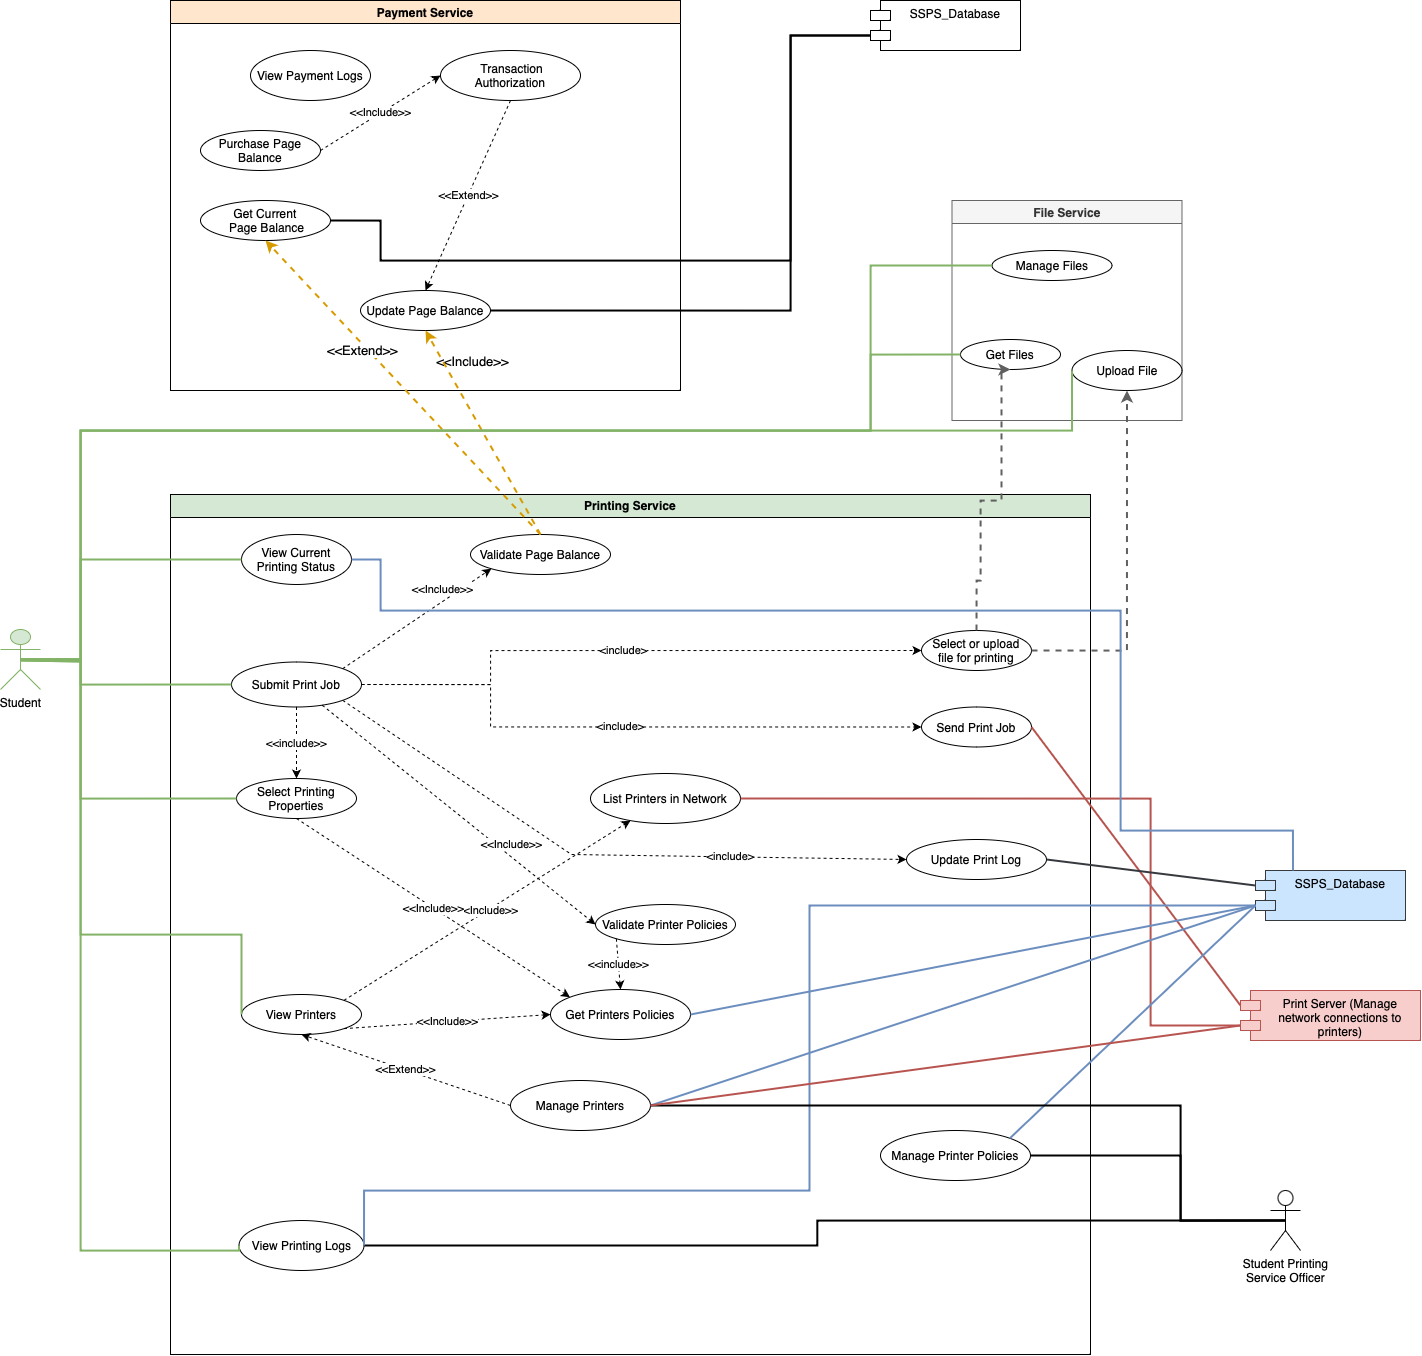
\includegraphics[max width=0.9\linewidth]{chapters/3. use-case-diagram/printing-use-case-diagram.png}
  \caption{Use case of the whole system}%
\end{figure}

\subsubsection{Table Format: Submit Print Job}

\begin{table}[H]
\begin{tabular}{|p{5cm}|p{9cm}|}
\hline
\textbf{Use Case Name} & Submit Print Job \\
\hline
\textbf{Actors} & Student User, Printing Service, Print Server, Payment Service, SSPS\_Database \\
\hline
\textbf{Description} & SPSO generates detailed reports at the end of each month and year, including total printed pages, page size breakdown, printer activity, student-specific logs, purchased pages summary, and system configuration changes. \\
\hline
\textbf{Trigger} & User clicks on "+ New Print" button on the sidebar  \\
\hline
\textbf{Preconditions} & User is logged in with an active user session. The document to be printed is uploaded and accessible. \\
\hline
\textbf{Postconditions} & The print job is successfully submitted for processing, and the user is notified when the print job is completed. \\
\hline
\textbf{Normal Flows} & 
1. User selects the desired printer for the print job. \\
&2. User selects the document to be printed. \\
&3. User specifies printing properties such as paper size, single-/double-sided, number of copies, and other preferences. \\
&4. User confirms the print job submission. \\
&5. System processes the print job and adds it to the print queue. \\
&6. User receives a confirmation message that the print job has been successfully submitted. \\
&7. User is notified when the print job is completed. \\
\hline
\end{tabular}
\caption{Submit Print Job}
\end{table}

\begin{table}[H]
\begin{tabular}{|p{5cm}|p{9cm}|}
\hline
\textbf{Alternative Flows} & 
\textbf{From 2a.} User clicks on Uploaded Files tab: \\
&2a.1. User clicks on their uploaded file from the list. \\
&2a.2. Proceed with step 3 and onwards as in the normal flow. \\
& \textbf{From 2b.} User clicks on Integrations tab: \\
&2b.1. User clicks on the integration button (e.g., Google Drive, OneDrive). \\
&2b.2. User follows the integration flow to select a file. \\
&2b.3. Proceed with step 3 and onwards as in the normal flow. \\
& \textbf{From 7b.} If the user runs out of page balance and chooses the Get More Balance button: \\
&7b.1. User clicks the "Get More Balance" button. \\
&7b.2. User is redirected to the page for adding more balance to their account. \\
&7b.3. Proceed with the balance addition process. \\
&7b.4. After successfully adding more balance, return to the print job confirmation step (step 4) and continue with the normal flow. \\
\hline
\textbf{Exceptions} & 
\textbf{From 5a.} If the selected printer is unavailable or offline, display an error message and allow the user to choose an alternative printer. \\
& \textbf{From 7a.} If the user runs out of page balance and chooses Cancel, display a notification and do not proceed with printing. \\
\hline
\end{tabular}
\caption{Submit Print Job (cont.)}
\end{table}

\subsection{Report Generation and Viewing}

\begin{figure}[H]
  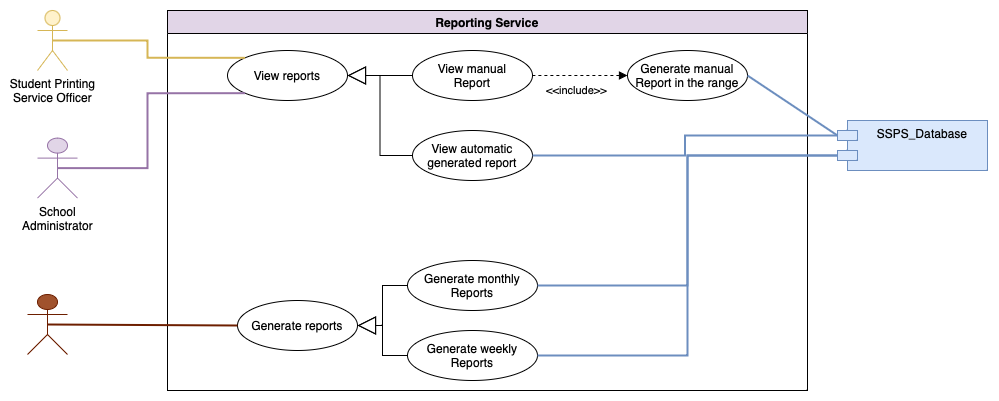
\includegraphics[max width=0.9\linewidth]{chapters/3. use-case-diagram/reporting-service.png}
  \caption{Use case of the whole system}%
\end{figure}

\subsubsection{Table Format: Generate Report}

\begin{table}[H]
\begin{tabular}{|p{5cm}|p{9cm}|}
\hline
\textbf{Use Case Name} & Report Generation \\
\hline
\textbf{Actors} & Student Printing Service Officer, School admin, Cron-job module, SSPS\_Database, Reporting Service \\
\hline
\textbf{Description} & SPSO generates detailed reports either on-demand by selecting a time range or through automated generation triggered by a cron job module. Reports include total printed pages, page size breakdown, printer activity, student-specific logs, purchased pages summary, and system configuration changes. \\
\hline
\textbf{Trigger} & - End of each month and year for automated generation. \\
& - SPSO is logged in and navigates to Report page and clicks on "Generate Report". \\
\hline
\textbf{Preconditions} & 1. SPSO is logged into the system. \\
& 2. For on-demand generation, SPSO selects "Reports" link from the sidebar. \\
\hline
\textbf{Postconditions} & 1. Reports for the specified time period are generated and stored. \\
\hline
\textbf{Normal Flows} & 1. "Generate Report" dialog is opened \\
& 2. SPSO selects the time range and report type. \\
& 3. SPSO initiates report generation. \\
& 4. The system generates and stores the report. \\
& 5. SPSO views and downloads the report. \\
\hline
\end{tabular}
\caption{Report Generation}
\end{table}

\begin{table}[H]
\begin{tabular}{|p{5cm}|p{9cm}|}
\hline
\textbf{Alternative Flows} & \textbf{From 1.} Cron job module triggers the generation of weekly and monthly reports. \\
& 1.1. The system generates and stores reports. \\
& 1.2. SPSO can access these reports at any time. \\
\hline
\textbf{Exceptions} & 1. If SPSO is not logged in, on-demand generation cannot proceed. \\
& 2. If no data is available for the specified time period, an empty report may be generated for on-demand or automated generation. \\
\hline
\end{tabular}
\caption{Report Generation (cont.)}
\end{table}

\subsubsection{Table Format: Report Viewing}

\begin{table}[H]
\begin{tabular}{|p{5cm}|p{9cm}|}
\hline
\textbf{Use Case Name} & View reports \\
\hline
\textbf{Actors} & Student Printing Service Officer, School admin, SSPS\_Database, Reporting Service\\
\hline
\textbf{Description} & Viewing the printing report \\
\hline
\textbf{Trigger} &SPSO navigates to Report page. \\
\hline
\textbf{Preconditions} & User is logged in with an active user session. User either has school administrator or SPSO role. \\
\hline
\textbf{Postconditions} & None \\
\hline
\textbf{Normal Flows} &1. The system find and list all reports from the database.\\
&2. The user selects one of the report link from the list.\\
&3. A dialog is shown and the user can view the rendered report \\
\hline
\textbf{Alternative Flows} & \textbf{From 1.} User clicks on Generate Report Manually button.\\
&1.2 User select the desired time range of the report.\\
&1.3 The report is then generated using the data got from the database.\\
&1.4 Continue from Step 3. in Normal Flows \\
&  \textbf{From 3.} User clicks on Download Report \\
&  3.1 The report is downloaded to the user device \\
\hline

\end{tabular}
\caption{View reports}
\end{table}